\documentclass[11pt]{article}

\usepackage[T1]{fontenc}
\usepackage{lmodern}
\usepackage[a4paper,margin=2.6cm]{geometry}
\usepackage{microtype}
\usepackage{amsmath,amssymb,amsthm,mathtools}
\usepackage{booktabs,array,tabularx}
\usepackage{xcolor}
\usepackage{listings}
\usepackage{tikz}
\usetikzlibrary{positioning,arrows.meta,calc}
\usepackage[hidelinks]{hyperref}
\usepackage[capitalise,nameinlink]{cleveref}

\definecolor{rocqkw}{rgb}{0.10,0.20,0.55}
\definecolor{rocqcm}{rgb}{0.35,0.35,0.35}
\lstdefinelanguage{Rocq}{
  morekeywords={Definition,Fixpoint,Lemma,Theorem,Proof,Qed,forall,exists,fun,match,
    with,end,let,in,Inductive,Prop,Type,Require,Import,From},
  sensitive=true,
  morecomment=[n]{(*}{*)},
}
\lstset{
  language=Rocq,
  basicstyle=\ttfamily\small,
  keywordstyle=\color{rocqkw}\bfseries,
  commentstyle=\color{rocqcm}\itshape,
  columns=fullflexible,
  keepspaces=true,
  xleftmargin=1.2em,
  aboveskip=0.8em,
  belowskip=0.8em,
  showstringspaces=false,
}

\theoremstyle{plain}
\newtheorem{theorem}{Theorem}[section]
\newtheorem{lemma}[theorem]{Lemma}
\newtheorem{proposition}[theorem]{Proposition}
\newtheorem{corollary}[theorem]{Corollary}
\theoremstyle{definition}
\newtheorem{definition}[theorem]{Definition}
\theoremstyle{remark}
\newtheorem{remark}[theorem]{Remark}

\newcommand{\N}{\mathbb{N}}
\newcommand{\T}[1]{T_{#1}}
\newcommand{\Prv}{\mathrm{Pr}}
\newcommand{\gn}[1]{\ulcorner #1 \urcorner}
\newcommand{\num}[1]{\overline{#1}}
\newcommand{\Sub}{\mathrm{Sub}}
\newcommand{\PSub}{\mathrm{PrSub}}
\newcommand{\Row}{\mathrm{Row}}
\newcommand{\Num}{\mathrm{Num}}
\newcommand{\Pat}{\mathrm{Pat}}
\newcommand{\PRI}{\mathrm{PI}}
\newcommand{\pair}[2]{\langle #1, #2\rangle}
\newcommand{\rocq}[1]{\texttt{#1}}
\setlength{\emergencystretch}{3em}
\newcommand{\sat}{\models}
\newcommand{\Ddelta}{\Delta_0}
\newcommand{\Ssigma}{\Sigma_1}

\title{Provable $\Sigma_1$-Completeness, Machine-Checked:\\
The Third Derivability Condition Derived inside Arithmetic}
\author{Charles C.\ Norton}
\date{September 2026}

\begin{document}
\maketitle

\begin{abstract}
We present a formalization, in the Rocq prover, of provable
$\Sigma_1$-completeness for a tower of arithmetic theories
$\T0 \subseteq \T1 \subseteq \cdots$ whose base $\T0$ has the axioms of
Robinson arithmetic and the induction schema.  For every level $k$ and
every $\Sigma_1$ formula $\sigma$ with free variables
$x_1,\dots,x_m$ we prove
\[
  \T0 \vdash \sigma(x_1,\dots,x_m) \to
  \Prv_k\bigl(\gn{\sigma(\dot x_1,\dots,\dot x_m)}\bigr),
\]
where $\Prv_k$ is the arithmetized provability predicate of $\T{k}$ and
the dotted substitution is computed inside arithmetic by an explicit
formula for numeral substitution into codes.  We also prove that this
formula means what it says: at every valuation $e$ it is true in $\N$
exactly when $\T{k}$ proves $\sigma$ with the numerals of
$e(x_1),\dots,e(x_m)$ substituted.  The third Hilbert--Bernays--L\"ob
derivability condition
$\T0 \vdash \Prv_k(\gn{A}) \to \Prv_k(\gn{\Prv_k(\gn{A})})$ follows as
the instance $\sigma := \Prv_k(\gn{A})$.  The proof carries the
textbook induction on $\Ddelta$ formulas out inside the object theory,
through a calculus of \emph{provable instances} of code patterns whose
slots hold numeral codes.  The development adds about 12{,}800 lines to
an existing formalization of the tower and its proof predicate, and the
theorems depend on no axiom beyond excluded middle.
\end{abstract}

\section{Introduction}\label{sec:intro}

Let $T$ be an arithmetic theory with a $\Sigma_1$ provability predicate
$\Prv_T$.  The Hilbert--Bernays--L\"ob derivability conditions
\cite{HilbertBernays1939,Loeb1955} are
\begin{description}
  \item[D1] if $T \vdash A$ then $T \vdash \Prv_T(\gn{A})$;
  \item[D2] $T \vdash \Prv_T(\gn{A \to B}) \to (\Prv_T(\gn{A}) \to \Prv_T(\gn{B}))$;
  \item[D3] $T \vdash \Prv_T(\gn{A}) \to \Prv_T(\gn{\Prv_T(\gn{A})})$.
\end{description}
Together with the diagonal lemma they yield L\"ob's theorem, G\"odel's
second incompleteness theorem, and the arithmetic soundness of the
provability logic GL \cite{Boolos1993,Smorynski1985}.  D1 is a meta-level
statement and follows from the $\Sigma_1$-completeness of the theory for
true sentences.  D2 is an internal statement about concatenating two
proofs.  D3 is the deep one: it asks the theory to prove, about its own
proof predicate, that whenever a proof exists this fact is itself
provable.  The standard route \cite{Boolos1993,HajekPudlak1993} derives
D3 from \emph{provable} $\Sigma_1$-completeness,
\begin{equation}\label{eq:main}
  T \vdash \sigma(x_1,\dots,x_m) \to
  \Prv_T\bigl(\gn{\sigma(\dot x_1,\dots,\dot x_m)}\bigr)
  \qquad (\sigma \in \Sigma_1),
\end{equation}
by taking $\sigma := \Prv_T(\gn{A})$, which is a $\Sigma_1$ sentence.
Here $\dot x$ denotes the numeral of the value of $x$, so the right-hand
side is the provability predicate applied to the code of $\sigma$ with
numerals substituted for its free variables, a term that the theory must
compute.

The textbook proof of \eqref{eq:main} is an induction on the structure of
$\sigma$, and it is usually given in a few pages.  Each step, however,
asserts the existence of an object-level derivation of a statement
\emph{about} the proof predicate, and the derivation must be produced
uniformly in the free variables.  In a formalization nothing about the
proof predicate is available except its definition: every syntactic
computation the argument performs on codes (substitution, occurrence
tests, the admissibility test for substitution, the construction of
numerals) has to be carried out \emph{inside} the object theory, on
codes denoted by variables, and every inference that the informal
argument makes ``under $\Prv$'' has to be justified by an explicit
object-level construction of a derivation.  Abstract formal accounts of
the incompleteness theorems accordingly take the derivability conditions
as hypotheses \cite{PopescuTraytel2019}.

This paper describes a complete machine-checked proof of \eqref{eq:main}
for every level of the arithmetic reflection tower of the
\rocq{provability-verified} development \cite{ProvabilityVerified},
the arithmetic layer of the \rocq{tiling-verified} formalization of the
polymodal provability calculus GLP* \cite{TilingVerified}.  Our main
results are the following, stated precisely in \cref{sec:statement}.
\begin{enumerate}
  \item \emph{Provable $\Sigma_1$-completeness with free variables}
    (\cref{thm:open}): for every level $k$ and every $\Sigma_1$ formula
    $\sigma$, $\T0 \vdash \sigma \to \PSub_k(\sigma)$, where
    $\PSub_k(\sigma)$ applies $\Prv_k$ to the output of an explicit
    formalized numeral-substitution function.
  \item \emph{Adequacy} (\cref{thm:meaning}): $\N, e \sat \PSub_k(\sigma)$
    if and only if $\T{k}$ proves $\sigma$ with the numerals of the
    values $e(x_i)$ substituted.  The statement of the main theorem is
    therefore self-interpreting: a reader need not inspect the
    arithmetization to know what is proved.
  \item \emph{The sentence form and D3} (\cref{cor:sentence,cor:d3}):
    $\T0 \vdash \sigma \to \Prv_k(\gn{\sigma})$ for $\Sigma_1$ sentences,
    and $\T0 \vdash \Prv_k(\gn{A}) \to \Prv_k(\gn{\Prv_k(\gn{A})})$.
  \item A \emph{proof architecture} that makes the internal induction
    tractable: code patterns with slots for numeral codes, a derived
    tag-3 substitution row for the code of any formula, and a calculus
    of provable instances with modus ponens, instantiation, existential
    elimination and case splitting (\cref{sec:proof}).
\end{enumerate}
All results are proved in Rocq~9.0 and depend on no axiom other than
the law of excluded middle.  Together with the internal second
derivability condition proved earlier in the same development, they
make the derivability conditions theorems of $\T0$ rather than axioms.

\paragraph{Outline.}
\Cref{sec:theory} fixes the object theory, the coding and the proof
predicate.  \Cref{sec:statement} states the theorems.
\Cref{sec:proof} explains the proof, from the rows of computation tables
up to the substitution chain and the adequacy theorem.
\Cref{sec:formal} describes the Rocq development and how to check it.
\Cref{sec:related} discusses related work, and \cref{sec:limits} the
limits of the result and the next steps.

\section{The object theory}\label{sec:theory}

\subsection{Language, substitution and formula classes}

Terms and formulas are built from variables $x_i$ ($i \in \N$), $0$,
successor $S$, $+$ and $\cdot$, with the primitive connectives $=$,
$\bot$, $\to$, $\forall$ and $\exists$; negation, conjunction and
disjunction are the usual abbreviations
$\neg A \equiv A \to \bot$, $A \wedge B \equiv \neg(A \to \neg B)$ and
$A \vee B \equiv \neg A \to B$.  The numeral of $n$ is
$\num{n} = S^n 0$.

Substitution $A[t/x]$ replaces the free occurrences of $x$ in $A$ by $t$
without renaming bound variables.  The calculus uses it only when it is
admissible: $\mathrm{adm}(x,t,A)$ holds when no free occurrence of $x$
in $A$ lies in the scope of a quantifier that binds a variable of $t$.
Numerals are closed, so substituting a numeral is always admissible.

The relation $v < t$ is expressed as $\exists v'\,(v + S v' = t)$ with
$v' = x_{i+1}$ when $v = x_i$, and bounded quantifiers are
\[
  (\forall v < t)\, A \;\equiv\; \forall v\,\bigl(v < t \to A\bigr),
  \qquad
  (\exists v < t)\, A \;\equiv\; \exists v\,\bigl(v < t \wedge A\bigr),
\]
where $v$ and its successor variable do not occur in $t$.  The class
$\Ddelta$ is the least class containing the equations and $\bot$ and
closed under $\to$ and bounded quantification; $\Ssigma$ is the closure
of $\Ddelta$ under existential quantification.

\subsection{The tower}

The theories $\T{n}$ are given by an inductive derivability relation
\rocq{FOProvesTn n}.  Every level has the axioms of Robinson arithmetic
$\mathsf{Q}$ and every instance of the induction schema
\[
  A[0/x] \to \forall x\,\bigl(A \to A[Sx/x]\bigr) \to \forall x\, A .
\]
In addition, for every $k < n$ the level $n$ has the local reflection
schema $\Prv_k(\gn{A}) \to A$, the schemes D2 and D3 for $\Prv_k$, and
the monotonicity scheme $\Prv_k(\gn{A}) \to \Prv_{k'}(\gn{A})$ for
$k \le k' < n$.  These level-restricted schemes are empty at $n = 0$, so
the axioms of $\T0$ are exactly those of $\mathsf{Q}$ and induction.
The rules are those of a Hilbert calculus for classical first-order
logic with equality (the combinators K and S, double negation, modus
ponens, generalization, equality and congruence axioms, universal
instantiation and existential introduction at admissible substitutions,
existential elimination, and distribution of $\forall$ over $\to$),
together with a L\"ob rule for the level's own predicate: from
$\T{n} \vdash \Prv_n(\gn{A}) \to A$ infer $\T{n} \vdash A$.  We return
to this rule in \cref{sec:limits}.

The base development establishes the following facts, which we use.
\begin{description}
  \item[Soundness] each level is sound: its theorems are true in $\N$
    under every valuation (\rocq{FOProvesTn\_sound});
  \item[Cumulativity] $\T{n} \vdash A$ implies $\T{m} \vdash A$ for
    $n \le m$ (\rocq{FOProvesTn\_cumulative});
  \item[Adequacy] $\N \sat \Prv_k(\gn{A})$ if and only if $\T{k} \vdash A$
    (\rocq{FOProvSentence\_sat\_iff});
  \item[D1] $\T{k} \vdash A$ implies $\T{m} \vdash \Prv_k(\gn{A})$ for
    every $m$ (\rocq{FOHBL3\_provable}), obtained from the
    $\Sigma_1$-completeness of $\mathsf{Q}$ for true closed $\Sigma_1$
    sentences;
  \item[D2] $\T0 \vdash \Prv_k(\gn{A \to B}) \to
    (\Prv_k(\gn{A}) \to \Prv_k(\gn{B}))$ (\rocq{FOHBL2\_internal}),
    derived inside $\T0$ by merging two checked derivations and their
    computation tables.
\end{description}

\subsection{G\"odel numbering}

Codes use the Cantor pairing
$\pair{a}{b} = \tfrac12 (a+b)(a+b+1) + b$, with terms on the left and
formulas on the right:
\begin{align*}
  \gn{x_i} &= \pair{0}{i}, & \gn{t = u} &= \pair{0}{\pair{\gn t}{\gn u}},\\
  \gn{0} &= \pair{1}{0}, & \gn{\bot} &= \pair{1}{0},\\
  \gn{St} &= \pair{2}{\gn t}, & \gn{A \to B} &= \pair{2}{\pair{\gn A}{\gn B}},\\
  \gn{t+u} &= \pair{3}{\pair{\gn t}{\gn u}}, & \gn{\forall x_i\, A} &= \pair{3}{\pair{i}{\gn A}},\\
  \gn{t \cdot u} &= \pair{4}{\pair{\gn t}{\gn u}}, & \gn{\exists x_i\, A} &= \pair{4}{\pair{i}{\gn A}}.
\end{align*}
The graph of pairing is defined by a $\Ddelta$ formula.

\subsection{Computation tables and the proof predicate}\label{sec:tables}

The syntactic operations on codes are represented by \emph{computation
tables}.  A table is a list of rows $(t, a_1, a_2, a_3, r)$ stored in
five columns through G\"odel's $\beta$-function
$\beta(c,d,i) = c \bmod (d(i+1)+1)$, so that a table of length $\ell$ is
given by eleven numbers.  The tag $t$ selects the operation the row
records:
\begin{center}
\begin{tabular}{@{}cl@{}}
\toprule
tag & the row $(t,a_1,a_2,a_3,r)$ records \\
\midrule
0 & $r = 1$ if the variable $x_{a_1}$ occurs in the term coded $a_2$, else $r=0$\\
1 & $r = 1$ if $x_{a_1}$ occurs free in the formula coded $a_2$, else $r=0$\\
2 & $r = \gn{t[s/x_{a_1}]}$ when $a_2 = \gn{s}$ and $a_3 = \gn{t}$\\
3 & $r = \gn{A[s/x_{a_1}]}$ when $a_2 = \gn{s}$ and $a_3 = \gn{A}$\\
4 & $r = 1$ if $\mathrm{adm}(x_{a_1}, s, A)$ when $a_2=\gn s$ and $a_3 = \gn A$, else $r=0$\\
5 & $r = \gn{\num{a_1}}$\\
\bottomrule
\end{tabular}
\end{center}
A table is \emph{valid} when every row satisfies the step clause for its
tag; the step clause decomposes the codes by pairing and refers to the
rows of the sub-computations, which must occur in the same table.
Validity is $\Ddelta$ in the eleven numbers.  Two facts connect tables
to the operations they represent: in a valid table every row is correct
(\rocq{tbl\_sound}), and every finite set of rows closed under the step
clauses is the set of rows of some valid table (\rocq{table\_realize}).
We write
\[
  \Row_t(a_1,a_2,a_3,r) \;:\equiv\; \exists T\,\bigl(\mathrm{Valid}(T)
  \wedge (t,a_1,a_2,a_3,r) \in T\bigr),
\]
a $\Ssigma$ formula (\rocq{FOTBLEX}).  Numeral codes are captured by
\[
  \Num(z,\mu) \;:\equiv\; \Row_5(z,0,0,\mu) \wedge
  \forall u\,\forall s\, \Row_2(u,s,\mu,\mu) \wedge
  \forall u\, \Row_0(u,\mu,0,0),
\]
which says that $\mu$ is the code of $\num{z}$ and records, as rows,
that substitution into $\mu$ changes nothing and that no variable occurs
in it (\rocq{FONUMR}).

The proof predicate of level $k$ is a $\Ssigma$ formula
$\mathrm{Prf}_k(u, c)$ (\rocq{FOPRMAT}): there are a valid table, a
$\beta$-coded sequence of formula codes $f_0,\dots,f_\ell$ and a
sequence of justification codes such that $f_\ell = c$, each entry is
justified as an axiom of $\T{k}$ or as the conclusion of a rule applied
to earlier entries, the syntactic side conditions of each justification
are read from rows of the table, and each entry passes a guard.  The
parameter $u$ is the code of the template itself; it is used to check
the justifications of L\"ob-rule entries and, through a list of
self-applied templates for the levels below $k$, of the level-restricted
axioms.  The level-$k$ provability formula is
\[
  \Prv_k(c) \;:\equiv\; \mathrm{Prf}_k(\num{\gn{\mathrm{Prf}_k}}, c),
\]
and $\Prv_k(\gn{A})$ denotes its instance at the numeral
$\num{\gn{A}}$ (\rocq{FOProvSentence}).

\section{Statements}\label{sec:statement}

\subsection{Formalized numeral substitution}

The right-hand side of \eqref{eq:main} applies $\Prv_k$ to a code that
depends on the values of the free variables.  The language has no
function symbol for substitution, so the code is described relationally.
The description has to be capture-free for every $\Sigma_1$ formula
$\sigma$, whatever the names of its variables; in particular the terms
standing for the values must not be captured by the bound variables of
$\Row$ and $\Num$.  We therefore let the values enter only through
equations.

\begin{definition}[Numeral substitution into a code]\label{def:sub}
Let $q$ be a variable index, $c$ and $r$ terms, $x_1,\dots,x_m$ variable
indices and $y_1,\dots,y_m$ terms.  Define $\Sub_q(c; \vec x; \vec y; r)$
by recursion on $m$:
\begin{align*}
  \Sub_q(c;\,;\,; r) &:\equiv c = r,\\
  \Sub_q(c; x\vec x; y\vec y; r) &:\equiv
    \exists a\, \exists \mu\, \exists z\, \bigl(
      z = y \wedge \Num(z,\mu) \wedge \Row_3(\num{x}, \mu, c, a) \wedge
      \Sub_{q+3}(a; \vec x; \vec y; r) \bigr),
\end{align*}
where $a$, $\mu$ and $z$ are the variables $x_q$, $x_{q+1}$ and
$x_{q+2}$ (\rocq{FOSUBNUMS}).
\end{definition}

Each step substitutes, for the variable $x$, the numeral of the value of
$y$ into the formula coded by the current code $c$: $z$ carries the
value, $\mu$ is the code of its numeral, and the tag-3 row gives the
code $a$ of the result.  The terms $\vec y$ occur only in the equations
$z = y$, so no binder of $\Row$ or $\Num$ can capture them, and the
chain variables $x_q, x_{q+1},\ldots$ are chosen above every variable of
$\sigma$.

\begin{definition}[Substituted provability]\label{def:psub}
For a formula $\sigma$ let $x_1 < \cdots < x_m$ be its free variables,
let $M$ be the largest index of a variable occurring in $\sigma$, and
let $Q = 2001 + M$.  Define
\[
  \PSub_k(\sigma) \;:\equiv\; \exists x_Q\,\bigl(
    \Sub_{Q+1}(\num{\gn{\sigma}}; \vec x; x_1,\dots,x_m; x_Q) \wedge
    \Prv_k(x_Q) \bigr)
\]
(\rocq{FOSubProv}).  In the notation of \eqref{eq:main},
$\PSub_k(\sigma)$ is $\Prv_k(\gn{\sigma(\dot x_1,\dots,\dot x_m)})$.
\end{definition}

The offset 2001 keeps the code variable and the chain away from the
variable ranges reserved for the internal bound variables of the
arithmetized operations, which all lie below 1000.

\subsection{Main results}

For a formula $A$, variables $x_1,\dots,x_m$ and terms $t_1,\dots,t_m$
write $A[t_1/x_1,\dots,t_m/x_m]$ for the sequential substitution
$(\cdots(A[t_1/x_1])\cdots)[t_m/x_m]$ (\rocq{FOsubsts}); for closed
$t_i$ it coincides with simultaneous substitution.

\begin{theorem}[Provable $\Sigma_1$-completeness]\label{thm:open}
For every level $k$ and every $\Sigma_1$ formula $\sigma$,
\[
  \T0 \vdash \sigma \to \PSub_k(\sigma).
\]
\end{theorem}

\begin{theorem}[Adequacy of the substituted predicate]\label{thm:meaning}
For every level $k$, every formula $\sigma$ with free variables
$x_1<\dots<x_m$, and every valuation $e$,
\[
  \N, e \sat \PSub_k(\sigma) \iff
  \T{k} \vdash \sigma\bigl[\num{e(x_1)}/x_1, \dots, \num{e(x_m)}/x_m\bigr].
\]
\end{theorem}

\begin{theorem}[Totality of the substitution]\label{thm:total}
For every formula $\sigma$,
\[
  \T0 \vdash \exists x_Q\, \bigl(\Sub_{Q+1}(\num{\gn{\sigma}}; \vec x; \vec x; x_Q)
  \wedge x_Q = x_Q\bigr).
\]
\end{theorem}

\begin{corollary}[Sentence form]\label{cor:sentence}
For every $\Sigma_1$ sentence $\sigma$,
$\T0 \vdash \sigma \to \Prv_k(\gn{\sigma})$.
\end{corollary}

\begin{corollary}[Third derivability condition]\label{cor:d3}
For every formula $A$ and level $k$,
$\T0 \vdash \Prv_k(\gn{A}) \to \Prv_k(\gn{\Prv_k(\gn{A})})$.
\end{corollary}

\Cref{cor:d3} is \cref{cor:sentence} at $\sigma := \Prv_k(\gn{A})$,
which is a $\Sigma_1$ sentence.  By cumulativity every statement proved
in $\T0$ also holds in each $\T{n}$.  The four results are collected in
one Rocq theorem:

\begin{lstlisting}
Theorem provable_sigma1_completeness : forall k,
  (forall A, FOsigma1 A -> FOProvesTn 0 (FOImplF A (FOSubProv k A))) /\
  (forall e A, FOsat e (FOSubProv k A) <->
     FOProvesTn k (FOsubsts A (fvs A) (map (fun x => FOnumeral (e x)) (fvs A)))) /\
  (forall A, FOsigma1 A -> (forall x, FOfree_in x A = false) ->
     FOProvesTn 0 (FOImplF A (FOProvSentence k A))) /\
  (forall A, FOProvesTn 0
     (FOImplF (FOProvSentence k A) (FOProvSentence k (FOProvSentence k A)))).
\end{lstlisting}

\Cref{thm:meaning} applies to every formula, not only to $\Sigma_1$
ones.  Combined with soundness it shows that \cref{thm:open} is the
familiar statement: at every valuation $e$ satisfying $\sigma$, the
theory $\T{k}$ proves the numeral instance of $\sigma$ at $e$.  The
formal content of \cref{thm:open} is stronger, since the implication is
a single theorem of $\T0$ with free variables, not a family of
statements about instances.

\section{The proof}\label{sec:proof}

\Cref{fig:architecture} shows the structure of the argument.  We first
derive, inside $\T0$, the table rows that the argument needs
(\cref{sec:rows}), then introduce code patterns and derive the
substitution rows for the code of an arbitrary formula
(\cref{sec:patterns}).  On top of these we build a calculus of provable
instances (\cref{sec:pi}), in which the arithmetic of numerals is
developed by internal induction (\cref{sec:arith}).  The $\Delta_0$
induction (\cref{sec:delta0}) and the $\Sigma_1$ step (\cref{sec:sigma1})
give the sentence form and D3.  The free-variable form follows from a
chain of substitution rows (\cref{sec:chain}), and adequacy from the
soundness of tables and the totality of the chain
(\cref{sec:adequacy}).

\begin{figure}[t]
\centering
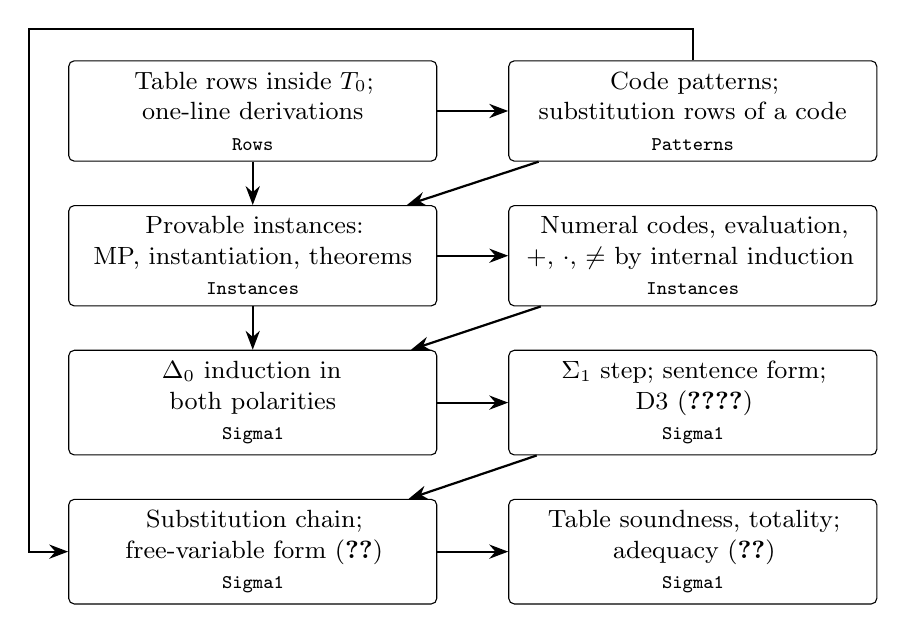
\begin{tikzpicture}[
  box/.style={draw, rounded corners=2pt, align=center, font=\small,
              inner sep=4pt, minimum height=2.6em, text width=12.5em},
  arr/.style={-{Stealth[length=2.4mm]}, thick},
  node distance=0.55cm and 0.9cm]
  \node[box] (rows) {Table rows inside $\T0$;\\ one-line derivations\\ \scriptsize\rocq{Rows}};
  \node[box, right=of rows] (pat) {Code patterns;\\ substitution rows of a code\\ \scriptsize\rocq{Patterns}};
  \node[box, below=of rows] (pi) {Provable instances:\\ MP, instantiation, theorems\\ \scriptsize\rocq{Instances}};
  \node[box, right=of pi] (arith) {Numeral codes, evaluation,\\ $+$, $\cdot$, $\neq$ by internal induction\\ \scriptsize\rocq{Instances}};
  \node[box, below=of pi] (d0) {$\Delta_0$ induction in\\ both polarities\\ \scriptsize\rocq{Sigma1}};
  \node[box, right=of d0] (s1) {$\Sigma_1$ step; sentence form;\\ D3 (\cref{cor:sentence,cor:d3})\\ \scriptsize\rocq{Sigma1}};
  \node[box, below=of d0] (chain) {Substitution chain;\\ free-variable form (\cref{thm:open})\\ \scriptsize\rocq{Sigma1}};
  \node[box, right=of chain] (adeq) {Table soundness, totality;\\ adequacy (\cref{thm:meaning})\\ \scriptsize\rocq{Sigma1}};
  \draw[arr] (rows) -- (pat);
  \draw[arr] (rows) -- (pi);
  \draw[arr] (pat) -- (pi);
  \draw[arr] (pi) -- (arith);
  \draw[arr] (pi) -- (d0);
  \draw[arr] (arith) -- (d0);
  \draw[arr] (d0) -- (s1);
  \draw[arr] (s1) -- (chain);
  \draw[arr] (pat.north) -- ++(0,0.4) -| ($(chain.west)+(-0.5,0)$) -- (chain.west);
  \draw[arr] (chain) -- (adeq);
\end{tikzpicture}
\caption{Structure of the proof and the Rocq file for each part.}
\label{fig:architecture}
\end{figure}

Throughout, $G \vdash A$ denotes derivability in $\T0$ from a finite
list $G$ of hypotheses; the deduction theorem makes this equivalent to
$\T0 \vdash \bigwedge G \to A$.  Many of the lemmas below carry side
conditions stating that certain variables are fresh; we omit them in the
exposition and describe the discipline that discharges them in
\cref{sec:formal}.

\subsection{Rows derived inside the theory}\label{sec:rows}

The argument never evaluates a table: every row it uses is derived
inside $\T0$ from rows of the sub-computations, by object-level
constructions of tables.  The basic operations are adding a row to a
valid table whose step clause is met by rows already present, and
joining the rows of two or three valid tables into one.  Both rely on
the object-level extension and concatenation of $\beta$-coded sequences
proved in the base development.

The same machinery yields \emph{one-line derivations}.  If an axiom
instance of $\T{k}$ has a justification whose side conditions are rows
(for instance, an instance of universal instantiation
$\forall x\,\theta \to \theta[t/x]$ requires a tag-3 row for
$\theta[t/x]$ and a tag-4 row with value 1), then $\T0$ derives
$\Prv_k$ of the instance's code from those rows: a one-entry derivation,
justified by the rows, witnesses the provability predicate.  These
derivations, D1 for closed theorems and the internal D2 are the only
ways in which the argument introduces $\Prv_k$.

\subsection{Code patterns}\label{sec:patterns}

Codes of formulas with numerals substituted for free variables are
described by patterns with slots.

\begin{definition}[Patterns]
Patterns are generated by $p ::= \mathsf{lit}\,n \mid \mathsf{slot}\,i
\mid \mathsf{succ}\,p \mid \mathsf{pair}\,p\,p$.  Given a list of terms
$\vec e$, the formula $\Pat_B(\vec e, p, d)$ states that $d$ is the value
of $p$ when $\mathsf{slot}\,i$ is filled by $e_i$
(\rocq{FOPATF}).  The intermediate values of the pairs are named by
bounded existential quantifiers over the variables $x_B, x_{B+1},\dots$,
so $\Pat$ is $\Ddelta$.
\end{definition}

For a partial map $\rho$ from variables to slot indices, the pattern
$\pi_\rho(A)$ of a formula $A$ is its code with each free variable $x$ in
the domain of $\rho$ replaced by $\mathsf{slot}\,\rho(x)$
(\rocq{cpat\_f}).  Every other variable contributes the literal code of
the variable, and bound variables are removed from $\rho$ under their
binder.  If the slots hold numeral codes $\gn{\num{n_i}}$, the value of
$\pi_\rho(A)$ is the code of $A$ with the numerals substituted.  Two
elementary lemmas are used everywhere: every pattern has a code,
$\T0 \vdash \exists d\, \Pat_B(\vec e, p, d)$, and the code is unique
(\rocq{FOPrH\_patf\_total}, \rocq{FOPrH\_patf\_unique}).

The central computational lemma derives the substitution row of a code
from the patterns of the source and the target.

\begin{lemma}[Substitution rows, \rocq{FOPrH\_rows\_f}]\label{lem:rows}
Let $x \notin \mathrm{dom}(\rho)$, let $\rho'$ extend $\rho$ by
$x \mapsto |\vec e|$, and suppose $G$ derives $\Num(w_i, e_i)$ for every
slot $i$ of $\vec e$.  Then
\[
  G, \Pat(\vec e, \pi_\rho(A), a), \Pat(\vec e s, \pi_{\rho'}(A), c)
  \vdash \Row_3(\num{x}, s, a, c).
\]
\end{lemma}

\begin{proof}[Proof sketch]
By induction on $A$, and on terms for the equations, using the tag-2
rows for terms.  At a slot the target and source codes coincide, and the
$\Num$ hypothesis supplies the row stating that substitution into a
numeral code leaves it unchanged.  At the variable $x$ itself the row
returns $s$.  At another literal variable $y$ the step clause needs
$\num{y} \neq \num{x}$, which is provable because $y \neq x$.  At a
binder the clause distinguishes whether the bound variable is $x$.  The
recursion is at the meta level and produces, for each $A$, an explicit
object-level derivation.
\end{proof}

\subsection{Provable instances}\label{sec:pi}

The textbook induction proves statements of the form ``if $\sigma$ holds
then $\Prv(\gn{\sigma(\dot{\vec x})})$''.  In our setting the code
$\gn{\sigma(\dot{\vec x})}$ is not a term, so we quantify over all codes
matching the pattern.

\begin{definition}[Provable instances, \rocq{PRI}]
For a hypothesis list $G$, a pattern $p$ and a list of numeral-code
terms $\vec e$, $\PRI(G, p, \vec e)$ holds if for every extension
$G' \supseteq G$ and every term $c$,
\[
  G' \vdash \Pat(\vec e, p, c) \quad\text{implies}\quad G' \vdash \Prv_k(c).
\]
\end{definition}

$\PRI$ is a meta-level property of object-level derivability, and the
quantification over extensions makes it stable under adding hypotheses,
which the existential eliminations below require.  The calculus has the
following rules.

\begin{lemma}[The calculus of provable instances]\label{lem:pi}
Let the slots of $\vec e$ hold numeral codes under $G$.
\begin{enumerate}
  \item \emph{Theorems} (\rocq{PRI\_thm}).  If $\T0 \vdash A$ and the free
    variables of $A$ lie in $\mathrm{dom}(\rho)$, then
    $\PRI(G, \pi_\rho(A), \vec e)$.
  \item \emph{Modus ponens} (\rocq{PRI\_mp}).  From
    $\PRI(G, \pi_\rho(A \to B), \vec e)$ and $\PRI(G, \pi_\rho(A), \vec e)$
    infer $\PRI(G, \pi_\rho(B), \vec e)$.
  \item \emph{Instantiation} (\rocq{PRI\_inst}).  If
    $\PRI(G, \pi_\rho(\forall x\,\theta), \vec e)$ and
    $G \vdash \Num(w, \mu)$, then
    $\PRI(G, \pi_{\rho'}(\theta), \vec e\mu)$ with
    $\rho' = \rho[x \mapsto |\vec e|]$.
  \item \emph{Existential elimination} (\rocq{PRI\_exe}).  If
    $G \vdash \exists x\, X$ and $\PRI(G \cup \{X[w/x]\}, p, \vec e)$ for a
    fresh variable $w$, then $\PRI(G, p, \vec e)$.
  \item \emph{Case split} (\rocq{PRI\_cases}).  If
    $\PRI(G \cup \{X\}, p, \vec e)$ and $\PRI(G \cup \{\neg X\}, p, \vec e)$,
    then $\PRI(G, p, \vec e)$.
  \item \emph{Reslotting} (\rocq{PRI\_reslot}).  If $\rho$ and $\rho'$
    assign to each free variable of $A$ slots whose contents are
    provably equal, then $\PRI(G,\pi_\rho(A),\vec e)$ implies
    $\PRI(G,\pi_{\rho'}(A),\vec e')$.
\end{enumerate}
\end{lemma}

\begin{proof}[Proof sketch]
(1) By D1, $\T0 \vdash \Prv_k(\gn{\forall \vec x A})$; iterated
instantiation (3) at the slot contents then gives the pattern of $A$.
(2) The code of $A \to B$ is $\pair{2}{\pair{a}{b}}$ for codes $a$ and
$b$ of the patterns, which exist by totality; the internal D2 applied at
these codes, with a guard row for the conclusion, gives $\Prv_k(c)$.
(3) The code of $\theta$ with the new slot is obtained from the code of
$\forall x\,\theta$ by the tag-3 row of \cref{lem:rows}; the admissibility
row has value 1 because the substituted code is a numeral code.  A
one-line derivation of the instantiation axiom and the internal D2
conclude.  (4) and (5) follow from the corresponding rules of the
calculus, because $\PRI$ quantifies over extensions of $G$.  (6) follows
because patterns with provably equal slot contents have provably equal
codes.
\end{proof}

\subsection{Arithmetic under the provability predicate}\label{sec:arith}

\paragraph{Numeral codes.}
$\T0$ proves $\forall z\, \exists \mu\, \Num(z,\mu)$ by induction on $z$,
the step adding the rows for $\gn{\num{z+1}} = \pair{2}{\gn{\num z}}$ to
a table.  Uniqueness follows by an internal induction, and inversion
($\Num(0,\mu) \to \mu = \gn{0}$;
$\Num(Sz,\mu) \to \exists \mu'\,(\Num(z,\mu') \wedge \mu = \pair{2}{\mu'})$)
by inverting the step clause of a tag-5 row.

\paragraph{Term evaluation.}
For every term $t$ whose variables have slots, and every fresh value
variable $z$ whose slot holds the numeral code of $t$,
$\PRI(G, \pi_\rho(t = z), \vec e)$ (\rocq{PRI\_teval}).  The proof is by
induction on $t$.  Variables and $0$ follow from theorems of the form
$x = x$, successors from the congruence theorem, and sums and products
from the next paragraph.

\paragraph{Sums, products and disequality by internal induction.}
The statement $\PRI(G, \pi(\num a + \num b = \num c), \vec e)$ for the
numeral codes of values $a$, $b$ and $c$ with $a + b = c$ cannot be
proved by a meta-level induction on $b$, because $b$ is the value of a
variable.  We internalize $\PRI$ for a fixed pattern as the formula
\[
  \mathrm{PI}^{\flat}(\vec e, p) \;:\equiv\; \forall c\,
  \bigl(\Pat(\vec e, p, c) \to \Prv_k(c)\bigr)
\]
(\rocq{PRIf}) and prove, by the induction schema of $\T0$, the formula
\[
  \Phi_+(N) \;:\equiv\; \forall \alpha\, \forall \beta\,
  \bigl(\Num(N, \alpha) \to \Num(x + N, \beta) \to
  \mathrm{PI}^{\flat}(\mu_x\alpha\beta, \pi(x_0 + x_1 = x_2))\bigr)
\]
for all $N$ (\rocq{PhiOp}, \rocq{PRI\_plus}).  The base case uses the
theorem $x + 0 = x$, and the step combines the induction hypothesis at
the inverted numeral code with the theorem
$x + y = z \to x + Sy = Sz$ under the provability predicate.  Products
are treated the same way over sums.  Disequality of numerals,
$\PRI(G, \pi(\neg\, \num a = \num b), \vec e)$ for $a \neq b$, is proved
by an internal induction on $a$ with the theorems $0 \neq Sy$,
$Sx \neq 0$ and $x \neq y \to Sx \neq Sy$ (\rocq{PhiNeq},
\rocq{PRI\_neq}).

\subsection{The \texorpdfstring{$\Delta_0$}{Delta-0} induction}\label{sec:delta0}

The induction over $\Delta_0$ formulas has to handle formulas whose free
variables are bound by quantifiers further out in $\sigma$.  We keep, for
every free variable $x$ of the current subformula, a \emph{holder}
variable $h(x)$ of $\T0$ above all variables of $\sigma$, a slot
$\rho(x)$, and a hypothesis $\Num(h(x), e_{\rho(x)})$ in the context;
$\mathrm{hsub}_h(A)$ denotes $A$ with each free $x$ renamed to $h(x)$.
The invariant \rocq{Inv} records these facts together with the freshness
bounds.

\begin{theorem}[$\Delta_0$ induction, \rocq{D0P\_all}]\label{thm:delta0}
For every $\Delta_0$ formula $A$ and every state $(G, h, \rho, \vec e)$
satisfying the invariant,
\begin{align*}
  G \vdash \mathrm{hsub}_h(A) &\;\Longrightarrow\; \PRI(G, \pi_\rho(A), \vec e),\\
  G \vdash \neg\,\mathrm{hsub}_h(A) &\;\Longrightarrow\;
  \PRI(G, \pi_\rho(\neg A), \vec e).
\end{align*}
\end{theorem}

\begin{proof}[Proof sketch]
By induction on $A$, proving both polarities together.
\begin{description}
  \item[Equations $t = u$.] Choose fresh value variables for $t$ and $u$
    with numeral codes by existential elimination.  Term evaluation gives
    $\PRI(\pi(t = z_1))$ and $\PRI(\pi(u = z_2))$.  In the positive case
    $G \vdash z_1 = z_2$, and the theorem
    $t = z \to u = z \to t = u$ concludes.  In the negative case the
    values differ, disequality gives $\PRI(\pi(\neg z_1 = z_2))$, and
    the theorem $t = z_1 \to u = z_2 \to \neg z_1 = z_2 \to \neg t = u$
    concludes.
  \item[$\bot$.] The positive case is vacuous by ex falso; the negative
    case is the theorem $\neg\bot$.
  \item[Implication $B \to C$.] In the positive case, split on
    $\mathrm{hsub}(B)$ inside the theory (\cref{lem:pi}(5)).  If it
    holds, $G \vdash \mathrm{hsub}(C)$, and the theorem
    $C \to (B \to C)$ applies.  If it fails, the negative hypothesis for
    $B$ gives $\PRI(\pi(\neg B))$, and the theorem
    $\neg B \to (B \to C)$ applies.  The negative case uses
    $B \to \neg C \to \neg(B \to C)$.
  \item[Bounded universals.] If
    $G \vdash (\forall v < t)\,\mathrm{hsub}(D)$, we prove by the
    induction schema of $\T0$, on the numeral bound $N$, the internal
    statement
    \[
      \Psi(N) :\equiv \forall \mu\,\bigl(\Num(N,\mu) \to
      (\forall v<N)\,\mathrm{hsub}(D) \to
      \mathrm{PI}^{\flat}(\vec e\mu, \pi((\forall v < y)\,D))\bigr),
    \]
    where $y$ is a fresh variable with the new slot (\rocq{BALL\_GEN}).
    The base case uses the theorem $(\forall v < 0)\,D$.  The step
    applies the induction hypothesis for $D$ at $v := N$, renamed to a
    slot by \rocq{cpat\_f\_subst\_var}, and the theorem
    $D[y/v] \to (\forall v<y)\,D \to (\forall v < Sy)\,D$.  Term
    evaluation for $t$ and the Leibniz theorem $t = y \to Q(y) \to Q(t)$
    then transfer the result from $y$ to $t$.  The negative case of
    bounded existentials is the same argument for $\neg D$.
  \item[Bounded existentials.] If $G \vdash (\exists v < t)\,\mathrm{hsub}(D)$,
    eliminate the witness, compute numeral codes for it and for the
    difference to $t$, derive $v + S w = t$ under the predicate by term
    evaluation, apply the induction hypothesis for $D$, and conclude with
    a theorem introducing the bounded existential (\rocq{WITNESS}).  The
    negative case of bounded universals is the same argument for
    $\neg D$.  \qedhere
\end{description}
\end{proof}

\subsection{The \texorpdfstring{$\Sigma_1$}{Sigma-1} step, the sentence form and D3}\label{sec:sigma1}

\begin{theorem}[$\Sigma_1$ induction, \rocq{S1P\_all}]\label{thm:s1}
For every $\Sigma_1$ formula $\sigma$ and every state satisfying the
invariant, $G \vdash \mathrm{hsub}_h(\sigma)$ implies
$\PRI(G, \pi_\rho(\sigma), \vec e)$.
\end{theorem}

\begin{proof}
For $\Delta_0$ formulas this is the positive half of \cref{thm:delta0}.
For $\exists x\, A$, eliminate the witness into a fresh holder $w_0$,
choose a numeral code $w_1$ for it, and extend the state by the slot for
$x$.  The induction hypothesis gives $\PRI$ for $A$ over
$\vec e w_1$.  The theorem $A \to \exists x\, A$, instantiated at the
slots, and modus ponens give $\PRI$ for $\exists x\,A$ over
$\vec e w_1$.  Reslotting removes the slot of $x$, which is not free in
$\exists x\,A$.
\end{proof}

For a $\Sigma_1$ sentence $\sigma$ take the context $[\sigma]$, the
identity holder map and no slots.  The pattern of a closed formula with
no slots is its literal code, so $\PRI([\sigma], \pi(\sigma), [\,])$ at
the code $\num{\gn\sigma}$ gives $[\sigma] \vdash \Prv_k(\gn{\sigma})$,
and the deduction theorem gives \cref{cor:sentence}.  \Cref{cor:d3} is
its instance at $\Prv_k(\gn{A})$, which is a closed $\Sigma_1$ formula.

\subsection{The substitution chain and the free-variable form}\label{sec:chain}

For a formula $\sigma$ with free variables $\vec x$ we work in the
context $[\mathrm{hsub}_h(\sigma)]$ with holders
$h(x) = H + x$ above the chain.  Existential elimination supplies
numeral codes $\mu_i$ with $\Num(h(x_i), \mu_i)$, and
\cref{thm:s1} gives $\PRI(\pi_\rho(\sigma), \vec\mu)$ for the map $\rho$
that sends $x_i$ to slot $i$.  By totality of patterns we name a code
$c$ of $\pi_\rho(\sigma)$ over $\vec\mu$, and $\PRI$ yields
$\Prv_k(c)$.  It remains to connect $c$ to the chain of
\cref{def:sub}.

\begin{lemma}[The chain, \rocq{SUBNUMS\_chain}]\label{lem:chain}
Suppose $G$ derives $\Num$ facts for the slots of $\vec e$ and
$\Num(y_i, \mu_i)$ for each $i$, together with
$\Pat(\vec e, \pi_\rho(A), a)$ and
$\Pat(\vec e\vec\mu, \pi_{\rho[\vec x \mapsto |\vec e|,\ldots]}(A), c)$,
where the variables $\vec x$ are outside $\mathrm{dom}(\rho)$.  Then
$G \vdash \Sub_q(a; \vec x; \vec y; c)$.
\end{lemma}

\begin{proof}
By induction on the list $\vec x$.  For the empty list, uniqueness of
pattern codes gives $a = c$.  For $x\vec x$, name the code $a'$ of the
pattern with the slot of $x$ filled by existential elimination.
\Cref{lem:rows} gives $\Row_3(\num x, \mu_1, a, a')$, and the induction
hypothesis at $a'$ gives the rest of the chain.  The three existential
quantifiers of the step are then introduced with the witnesses $a'$,
$\mu_1$ and $y_1$.
\end{proof}

Applied with $\rho$ empty, $\vec e$ empty and the literal code
$a = \num{\gn\sigma}$, the lemma gives
$\Sub(\num{\gn\sigma}; \vec x; h(\vec x); c)$ in the context
$[\mathrm{hsub}_h(\sigma)]$.  Existential introduction at $c$ then gives
the holder form of $\PSub_k(\sigma)$, and the deduction theorem gives
$\T0 \vdash \mathrm{hsub}_h(\sigma) \to \PSub_k(\sigma)[h(\vec x)/\vec x]$.
Finally the holders are renamed back to the variables one at a time, by
generalization and instantiation (\rocq{rename\_all}).  Each
instantiation is admissible because the free occurrences of $h(x)$ sit
exactly where $x$ occurs free in $\sigma$, and in $\PSub$ only inside
the equations $z = y$ of the chain.  This proves \cref{thm:open}.

\subsection{Adequacy}\label{sec:adequacy}

\begin{proposition}[Soundness of the chain, \rocq{SUBNUMS\_sound}]
If $\N, e \sat \Sub_q(c; \vec x; \vec y; r)$ and $e(c) = \gn{A}$, then
$e(r) = \gn{A[\num{e(y_1)}/x_1,\dots,\num{e(y_m)}/x_m]}$.
\end{proposition}

\begin{proof}
A true $\Row_t$ fact provides a valid table containing the row, and table
soundness gives the row's meaning.  Along the chain, the tag-5 row inside
$\Num$ identifies $\mu$ as the code of the numeral of the value of $y$,
and the tag-3 row identifies the next code as the code of the
substituted formula.  The chain variables are fresh for $c$, $r$ and
$\vec y$, so the updates of the valuation along the chain do not change
their values.
\end{proof}

\Cref{thm:total} is proved like \cref{thm:open}, with the trivially
derivable hypothesis $\sigma \to \sigma$ in place of $\sigma$ and the
equation $x_Q = x_Q$ in place of $\Prv_k(x_Q)$.  To prove
\cref{thm:meaning}, note first that
$\N, e \sat \Prv_k(x_Q)$ if and only if
$\N, e \sat \Prv_k(\num{e(x_Q)})$, by the semantic substitution lemma.
If $\PSub_k(\sigma)$ is true at $e$, the witness for $x_Q$ is the code of
the numeral instance by soundness of the chain, so $\Prv_k$ of that code
is true, and adequacy of $\Prv_k$ gives the $\T{k}$-derivation.
Conversely, soundness of $\T0$ applied to \cref{thm:total} provides a
witness for the chain at $e$, which is the code of the numeral instance,
and adequacy of $\Prv_k$ turns the assumed $\T{k}$-derivation into the
truth of $\Prv_k$ at that witness.

\section{The formalization}\label{sec:formal}

\subsection{Files and checking}

The work consists of the last four files in the \rocq{theories}
directory of the \rocq{provability-verified} development
\cite{ProvabilityVerified}, placed after the files that define the
syntax, the semantics, the proof checker and the internal second
derivability condition (\cref{tab:files}).  With Rocq~9.0,
\verb|make check| builds the development and re-validates it with
\verb|rocqchk|, which is what the repository's continuous integration
runs.  \verb|Print Assumptions provable_sigma1_completeness| reports the
single axiom \rocq{Classical\_Prop.classic}.

\begin{table}[t]
\centering
\begin{tabular}{@{}lrrrp{6.1cm}@{}}
\toprule
File & Lines & Stmts & Time & Content \\
\midrule
\rocq{Rows} & 2{,}952 & 98 & 987\,s & tables holding given rows, guard rows, one-line derivations, step clauses from component facts \\
\rocq{Patterns} & 2{,}892 & 84 & 133\,s & patterns of terms and formulas, their totality and uniqueness, substitution, occurrence and capture rows of a code \\
\rocq{Instances} & 3{,}769 & 146 & 240\,s & provable instances and their calculus, numeral codes, term evaluation, sums, products, disequality \\
\rocq{Sigma1} & 3{,}181 & 107 & 34\,s & $\Delta_0$ and $\Sigma_1$ inductions, sentence form, D3, substitution chain, adequacy, the summary theorem \\
\midrule
total & 12{,}794 & 435 & 1{,}394\,s & \\
\bottomrule
\end{tabular}
\caption{The files of this work, with their \texttt{Theorem}, \texttt{Lemma} and \texttt{Corollary} declarations and their compilation times with \texttt{coqc} on a laptop.}
\label{tab:files}
\end{table}

\subsection{Engineering}

\paragraph{Derivations under hypotheses.}
All object-level reasoning is done in the relation
$\rocq{FOPrH}\ n\ G\ A$, derivability of $A$ in $\T{n}$ from a list $G$
of hypotheses.  It is defined as provability of the iterated implication
and comes with introduction and elimination rules for the connectives
and quantifiers, including existential elimination at a fresh name and
the induction rule.  This lets the Rocq proofs follow the informal
natural-deduction style of \cref{sec:proof}.

\paragraph{Variable discipline.}
Naive substitution and fixed internal variable names make freshness the
dominant source of side conditions.  The development partitions the
variables.  The internal bound variables of the arithmetized operations
lie below 1000: the tables and their lookups use the indices 2 to 50,
the universal closures in $\Num$ the indices 802 to 804, and the
provability matrix the indices below 252.  Pattern bases, the variables
of the internal inductions and the holders use indices of at least 1000,
allocated upward from a bound $V$ that grows as fresh names are taken.  Most side
conditions are then linear inequalities between indices, discharged by
\texttt{lia}.  The rest (a variable does not occur in a term, is not
free in a formula, or a substitution is admissible) are discharged by a
small family of tactics that decompose formulas built from the
arithmetized operations and look up bounds stated as hypotheses.

\paragraph{Derivations as data.}
Object-level derivability is the inductive relation
\rocq{FOProvesTn}, so each theorem of the form $\T0 \vdash A$ denotes a
derivation tree in the Hilbert calculus of \cref{sec:theory}.  The
meta-level inductions of \cref{sec:proof} are ordinary Rocq inductions
that build these trees, uniformly in the formula they are applied to.

\section{Related work}\label{sec:related}

Shankar \cite{Shankar1994} checked G\"odel's first incompleteness
theorem with the Boyer--Moore prover, and O'Connor
\cite{OConnor2005} verified the essential incompleteness of arithmetic
in Coq.  Neither needs the derivability conditions.  Paulson
\cite{Paulson2014,Paulson2015} formalized both incompleteness theorems
in Isabelle/HOL for the theory of hereditarily finite sets, following
{\'S}wierczkowski \cite{Swierczkowski2003}.  His proof of the second
theorem establishes the derivability conditions for that theory,
including an internal form of $\Sigma$-completeness.  For arithmetic,
the Lean~4 library Foundation \cite{Foundation} proves the second
incompleteness theorem for $\Delta_1$-definable theories extending
$\mathsf{I}\Sigma_1$, with formalized $\Sigma_1$-completeness, including
its form for formulas with free variables, and the third derivability
condition $\mathsf{I}\Sigma_1 \vdash \Box\sigma \to \Box\Box\sigma$.
Its proofs reason inside an arbitrary model of $\mathsf{I}\Sigma_1$, in
which syntax and provability are internalized, and pass to derivability
through the completeness theorem.  The present development is
proof-theoretic instead: every step is an explicit derivation in the
Hilbert calculus of $\T0$, carried out on codes denoted by object-level
variables, with the provability predicate defined through
$\beta$-coded computation tables.  It also covers a tower of predicates
$\Prv_k$, states the numeral substitution as an explicit formula whose
standard-model meaning is proved, and is written in Rocq.  Popescu and
Traytel
\cite{PopescuTraytel2019} give an abstract account of the incompleteness
theorems that takes the derivability conditions as hypotheses and
instantiate it with Paulson's development.  Kirst and Hermes
\cite{KirstHermes2021} and Kirst and Peters \cite{KirstPeters2023}
develop synthetic approaches to undecidability and incompleteness in
Coq, which avoid arithmetized proof predicates altogether.

On the mathematical side, the derivability conditions go back to
Hilbert and Bernays \cite{HilbertBernays1939} and L\"ob
\cite{Loeb1955}, arithmetization in a general setting to Feferman
\cite{Feferman1960}, and the proof of provable $\Sigma_1$-completeness
we follow is the standard one of the textbooks
\cite{Boolos1993,Smorynski1985,HajekPudlak1993}.  The tower
$\T0 \subseteq \T1 \subseteq \cdots$ is the arithmetic setting of the
polymodal provability logics studied by Japaridze and Beklemishev
\cite{Beklemishev2005}, and the development it belongs to is motivated
by the L\"obian obstacle for self-modifying agents
\cite{YudkowskyHerreshoff2013}.

\section{Limits and next steps}\label{sec:limits}

\paragraph{The L\"ob rule.}
The calculus of the tower, as defined in the base development, closes
each level under a primitive L\"ob rule for its own predicate.  The rule
is sound, since every theorem of every level is true in $\N$, and the
axioms of $\T0$ are exactly those of $\mathsf{Q}$ and induction.  The
statement of \cref{thm:open} is nevertheless about $\T0$ as defined,
including the rule, and our development does not certify that the
derivations it constructs avoid it.  The next stage of the development
formalizes the diagonal lemma, L\"ob's theorem and the internal
monotonicity $\Prv_k(\gn{A}) \to \Prv_{k'}(\gn{A})$ for $k \le k'$.  It
then removes the primitive rule and the
level-restricted D2, D3 and monotonicity schemes, the first two of which
are already redundant by the internal proofs, so that $\T0$ is Peano
arithmetic and $\T{n+1}$ is $\T{n}$ plus local reflection for $\T{n}$.  The present results are stated for the tower as it is
defined now, and they will be re-established for the reduced tower.

\paragraph{Scope.}
The meaning theorem (\cref{thm:meaning}) makes the formalized
substitution trustworthy without inspecting the tables.  The truth of
the main theorem's statement still rests on the definitions of the
object theory, the coding and the $\Sigma_1$ class, which a reader has
to check against their informal counterparts.  These definitions are
short and are collected in the file \rocq{theories/Syntax.v}.

\section{Conclusion}

Provable $\Sigma_1$-completeness is where the arithmetization of
syntax has to be used \emph{inside} the theory rather than merely
defined, and it is the step that informal expositions most often
compress.  We have given a complete machine-checked proof for every
level of an arithmetic reflection tower, with free variables handled by
an explicit numeral-substitution formula whose meaning is itself
proved.  The third derivability condition follows as a corollary.
Code patterns with numeral-code slots, and the calculus of provable
instances built on them, reduce the internal induction to local
reasoning steps.  With D2 proved earlier, D1 is a derived rule of every
level, and D2 and D3 are theorems of the base theory.

\bibliographystyle{plain}
\begin{thebibliography}{99}

\bibitem{Beklemishev2005}
L.~D. Beklemishev.
\newblock Reflection principles and provability algebras in formal
  arithmetic.
\newblock \emph{Russian Mathematical Surveys}, 60(2):197--268, 2005.

\bibitem{Boolos1993}
G.~Boolos.
\newblock \emph{The Logic of Provability}.
\newblock Cambridge University Press, 1993.

\bibitem{Feferman1960}
S.~Feferman.
\newblock Arithmetization of metamathematics in a general setting.
\newblock \emph{Fundamenta Mathematicae}, 49:35--92, 1960.

\bibitem{Foundation}
FormalizedFormalLogic.
\newblock Foundation: formalization of mathematical logic in {L}ean~4.
\newblock \url{https://github.com/FormalizedFormalLogic/Foundation},
  2023--2026.

\bibitem{HajekPudlak1993}
P.~H{\'a}jek and P.~Pudl{\'a}k.
\newblock \emph{Metamathematics of First-Order Arithmetic}.
\newblock Springer, 1993.

\bibitem{HilbertBernays1939}
D.~Hilbert and P.~Bernays.
\newblock \emph{Grundlagen der Mathematik}, volume~II.
\newblock Springer, 1939.

\bibitem{KirstHermes2021}
D.~Kirst and M.~Hermes.
\newblock Synthetic undecidability and incompleteness of first-order axiom
  systems in {Coq}.
\newblock In \emph{12th International Conference on Interactive Theorem
  Proving (ITP 2021)}, volume 193 of \emph{LIPIcs}, 2021.

\bibitem{KirstPeters2023}
D.~Kirst and B.~Peters.
\newblock G{\"o}del's theorem without tears: essential incompleteness in
  synthetic computability.
\newblock In \emph{31st EACSL Annual Conference on Computer Science Logic
  (CSL 2023)}, volume 252 of \emph{LIPIcs}, 2023.

\bibitem{Loeb1955}
M.~H. L{\"o}b.
\newblock Solution of a problem of {L}eon {H}enkin.
\newblock \emph{The Journal of Symbolic Logic}, 20(2):115--118, 1955.

\bibitem{OConnor2005}
R.~O'Connor.
\newblock Essential incompleteness of arithmetic verified by {Coq}.
\newblock In \emph{Theorem Proving in Higher Order Logics (TPHOLs 2005)},
  volume 3603 of \emph{Lecture Notes in Computer Science}, pages 245--260.
  Springer, 2005.

\bibitem{Paulson2014}
L.~C. Paulson.
\newblock A machine-assisted proof of {G}{\"o}del's incompleteness theorems
  for the theory of hereditarily finite sets.
\newblock \emph{The Review of Symbolic Logic}, 7(3):484--498, 2014.

\bibitem{Paulson2015}
L.~C. Paulson.
\newblock A mechanised proof of {G}{\"o}del's incompleteness theorems using
  {N}ominal {I}sabelle.
\newblock \emph{Journal of Automated Reasoning}, 55(1):1--37, 2015.

\bibitem{PopescuTraytel2019}
A.~Popescu and D.~Traytel.
\newblock A formally verified abstract account of {G}{\"o}del's
  incompleteness theorems.
\newblock In \emph{Automated Deduction -- CADE 27}, volume 11716 of
  \emph{Lecture Notes in Computer Science}, pages 442--461. Springer, 2019.

\bibitem{Shankar1994}
N.~Shankar.
\newblock \emph{Metamathematics, Machines, and {G}{\"o}del's Proof}.
\newblock Cambridge University Press, 1994.

\bibitem{Smorynski1985}
C.~Smory{\'n}ski.
\newblock \emph{Self-Reference and Modal Logic}.
\newblock Springer, 1985.

\bibitem{Swierczkowski2003}
S.~{\'S}wierczkowski.
\newblock Finite sets and {G}{\"o}del's incompleteness theorems.
\newblock \emph{Dissertationes Mathematicae}, 422:1--58, 2003.

\bibitem{ProvabilityVerified}
C.~C. Norton.
\newblock provability-verified: provability in arithmetic, machine-checked in
  {R}ocq.
\newblock \url{https://github.com/CharlesCNorton/provability-verified}, 2026.

\bibitem{TilingVerified}
C.~C. Norton.
\newblock tiling-verified: a {R}ocq formalization of the polymodal
  provability calculus {GLP*} and its arithmetic tower.
\newblock \url{https://github.com/CharlesCNorton/tiling-verified}, 2026.

\bibitem{YudkowskyHerreshoff2013}
E.~Yudkowsky and M.~Herreshoff.
\newblock Tiling agents for self-modifying {AI}, and the {L}{\"o}bian
  obstacle.
\newblock Technical report, Machine Intelligence Research Institute, 2013.

\end{thebibliography}

\appendix

\section{Rocq statements}\label{app:statements}

The definitions of the formalized substitution and of the substituted
provability formula:

\begin{lstlisting}
Fixpoint FOSUBNUMS (q : nat) (c : FOTerm) (xs : list nat) (ys : list FOTerm)
    (r : FOTerm) : FOFormula :=
  match xs, ys with
  | x :: xs', y :: ys' =>
      FOExists q (FOExists (S q) (FOExists (S (S q))
        (FOAnd (FOEq (FOVar (S (S q))) y)
          (FOAnd (FONUMR (FOVar (S (S q))) (FOVar (S q)))
            (FOAnd (FOTBLEX (FOnumeral 3) (FOnumeral x) (FOVar (S q)) c (FOVar q))
                   (FOSUBNUMS (S (S (S q))) (FOVar q) xs' ys' r))))))
  | _, _ => FOEq c r
  end.

Definition FOSubProv (k : nat) (A : FOFormula) : FOFormula :=
  SPF (subq A) (FOnumeral (FOcode_f A)) (fvs A) (map FOVar (fvs A))
    (FOPRu (FOPrCores k) (FOu0 k) (FOVar (subq A))).
\end{lstlisting}
Here \rocq{SPF Q c xs ys R} is
\rocq{FOExists Q (FOAnd (FOSUBNUMS (S Q) c xs ys (FOVar Q)) R)},
\rocq{subq A} is \rocq{2001 + FOvars\_max A}, \rocq{fvs A} lists the free
variables of \rocq{A} in increasing order, and
\rocq{FOPRu (FOPrCores k) (FOu0 k) c} is $\Prv_k(c)$, which coincides
with \rocq{FOProvSentence k A} at \rocq{c = FOnumeral (FOcode\_f A)}.

The provable instances of a pattern:

\begin{lstlisting}
Definition PRI (n : nat) (cores : list nat) (u0 V : nat) (G : list FOFormula)
    (p : CPat) (env : list FOTerm) : Prop :=
  forall G' B c, (forall X, In X G -> In X G') -> FOctx_avoid G' 0 1000 ->
  FOtms_avoid [c] 0 1000 -> V <= B -> Clean G' [c] B ->
  FOPrH n G' (FOPATF B env p c) -> FOPrH n G' (FOPRu cores u0 c).
\end{lstlisting}

The $\Delta_0$ and $\Sigma_1$ inductions:

\begin{lstlisting}
Theorem D0P_all : forall n k W A, FOdelta0 A -> D0P n k W A.
Theorem S1P_all : forall n k W A, FOsigma1 A -> S1P n k W A.
\end{lstlisting}

\end{document}
